\section{Atomic Bonded Cross-chain Debt}
\label{sec:abcd}

Since the Alice's time's up transaction in the ABD primitive needs to be shared in both Alice's and Bob's stages, this form of bond can not be used across different blockchains. To solve the problem of interoperability for the atomic bond\new{,} we have redesigned our model using check-sequence-verify\footnote{The up-code CHECKSEQVERIFY}. In this section, we first build an intermediary component that has the same functionality as ABD. After that, we introduce \new{ABCD} that can be actually used between different blockchains.
% At the time of writing, there are more than a thousand implemented blockchains working. One of our concerns about the non-collateralized bond component is the possibility of using checkseqverify. If a blockchain does not support this type of opcode we can not use this type of bond in it.
Using the check-sequence-verify, the minimum amount of coins for the determinator transaction and the delay keeper stage are removed from the component.
% Using the "check sequence verify" there is no need for delay keeper stage and temp transaction and the minimum amount of coins used in the previous type.
\begin{figure}[h]
  \centering
  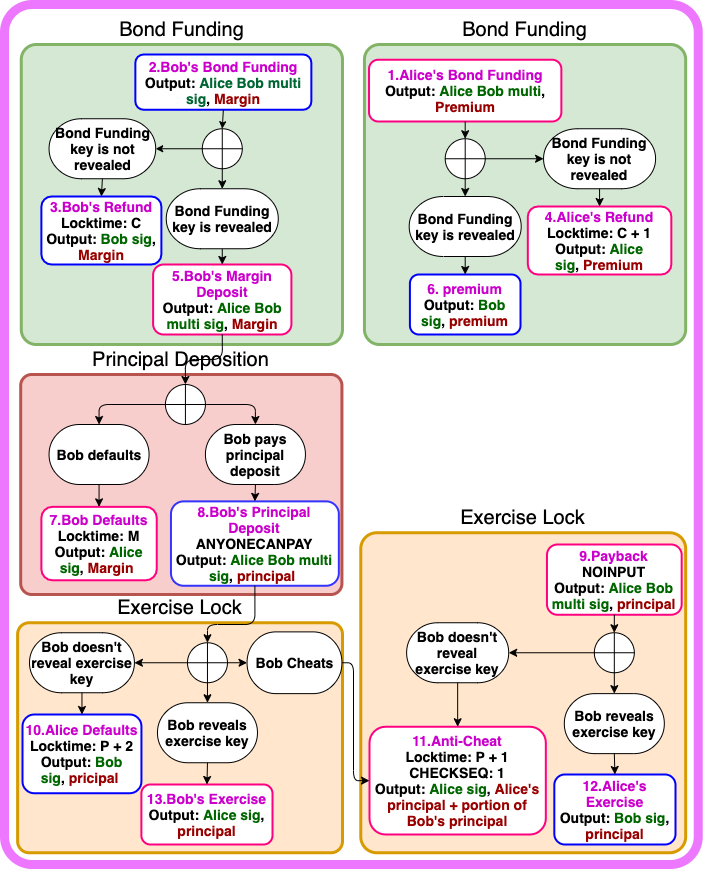
\includegraphics[width=\linewidth]{figures/bond-second.png}
  \caption{The ABD component using checkseq. On each transaction, signatures, output amount and locktimes are specified. All outputs are in the same coin. Pink-bordered transactions are broadcast by Alice and blue-bordered ones by Bob. For locktimes, block height is used. Upper transactions are broadcast earlier than the lower ones. If there is a line between two transactions, then the source transaction is considered to be an input of the destination transaction.}
  \Description{An atomic bonded debt using checkseqverify}
  \label{fig:non-collat-bond}
\end{figure}

The intermediary ABD component is demonstrated in Fig\new{.}~\ref{fig:non-collat-bond}. To present this type of ABD we use block height as the locktime parameter, however the Unix timestamp can also be used. The procedure is discussed below:

\begin{itemize}
    \item \textbf{Bond Funding}: Alice's funding includes premium and Bob's includes margin. \new{The number $C$ is the minimum} \new{number of mined blocks for a transaction} \new{to be confirmed.}
    
    \item \textbf{Principal Deposition}: 
        After issuing the bond, similar to the original ABD, each party has to deposit his principal within a specified time interval: Bob $M$ locktime and Alice $P$ ($P > M$). Bob's principal deposit transaction has sighash type of anyone-can-pay but Alice's \new{redemption} has \new{``}no-input" type since one of Bob's inputs is determined while none of Alice's inputs is clear at the time of creating the transaction. Bob can behave in one of the two following ways:
    \begin{itemize}
        \item He defaults, then Alice takes his margin by broadcasting the Bob defaults transaction.
        \item He deposits the principal, then the procedure goes to the next stage.
    \end{itemize}
    
    \item \textbf{Exercise Lock}: If Bob deposits his principal before the locktime, Alice has time before a $P$ locktime expires to \new{repurchase} her \new{bond}. As mentioned earlier, the \new{redemption} transaction has sighash type of no-input. The \new{``}checkseq 1" in the anti-cheat transaction, forces this transaction to have a minimum block distance of 1 from its parent i.e. the anti-cheat transaction can only be mined in a block with a higher block height than the block which Alice's \new{redemption} transaction is in, hence Bob has enough time to reveal the \keyone key. Note that the 1 block height difference may have to vary in different blockchains. For example in bitcoin, the minimum block height needed to elapse for the transactions to be confirmed is 6 blocks. Thus, we have to use \new{``}checkseq 6" in bitcoin. However, in this context, we assume the general case of 1 block.
    
    After Bob's principal deposition, there are two possible scenarios: 
    \begin{itemize}
        \item Alice succeeds to \new{repurchase}. Bob reveals the \keyone key. The result is similar to the original ABD. 
        
        \item Alice does not broadcast the \new{redemption} transaction hence Bob avoids exposing the \keyone key and his principal is sent back to himself. To achieve this, Bob gives Alice $P + 2$ locktime to convince him to reveal the \keyone key and if this deadline is passed, he will broadcast the Alice defaults transaction which gives him back his principal.
        
        \item Alice fulfills her \new{redemption} transaction but Bob does not reveal the \keyone key. In this case, Alice can broadcast the anti-cheat transaction to get her principal and a portion of Bob's principal as the punishment. Note that, since the anti-cheat transaction has a locktime of $P + 1$ and a checkseq of 1 and the Alice's defaults transaction has a locktime of $P + 1$, Alice has to broadcast her \new{redemption transaction} before $P$. Otherwise, she would not have enough time to broadcast the anti-cheat transaction in the case of Bob cheating. In other words, if the Alice's \new{redemption} transaction is mined in a block of at least $P + 1$ height and Bob does not reveal \keyone key, she can not get the anti-cheat transaction mined before block $P + 2$. Therefore, Bob can broadcast the Alice defaults in the $P + 1$th block and avoid giving her the capital.
    \end{itemize}
\end{itemize}

The reason which prevents the intermediary ABD component to be used in a cross-chain environment is that the anti-cheat transaction has inputs from both Alice's and Bob's sides. To overcome this issue, before exploiting any bond contract, Bob, which is considered to be an exchange or somebody who has a reasonable amount of assets in different blockchains, can deposit some assets as a bond guarantee in any desired chain. This way, Bob can offer his customers a cross-chain bond service that accepts his payback \new{on} the other chain. This modification can be seen in Fig.\ref{fig:cross-chain-non-collat-bond}. In \abcd, we use Unix timestamp for locktimes and we consider the maximum time among all of involved blockchains since in different blockchains the number of blocks needed for confirmation is different.


\begin{figure}[]
  \centering
  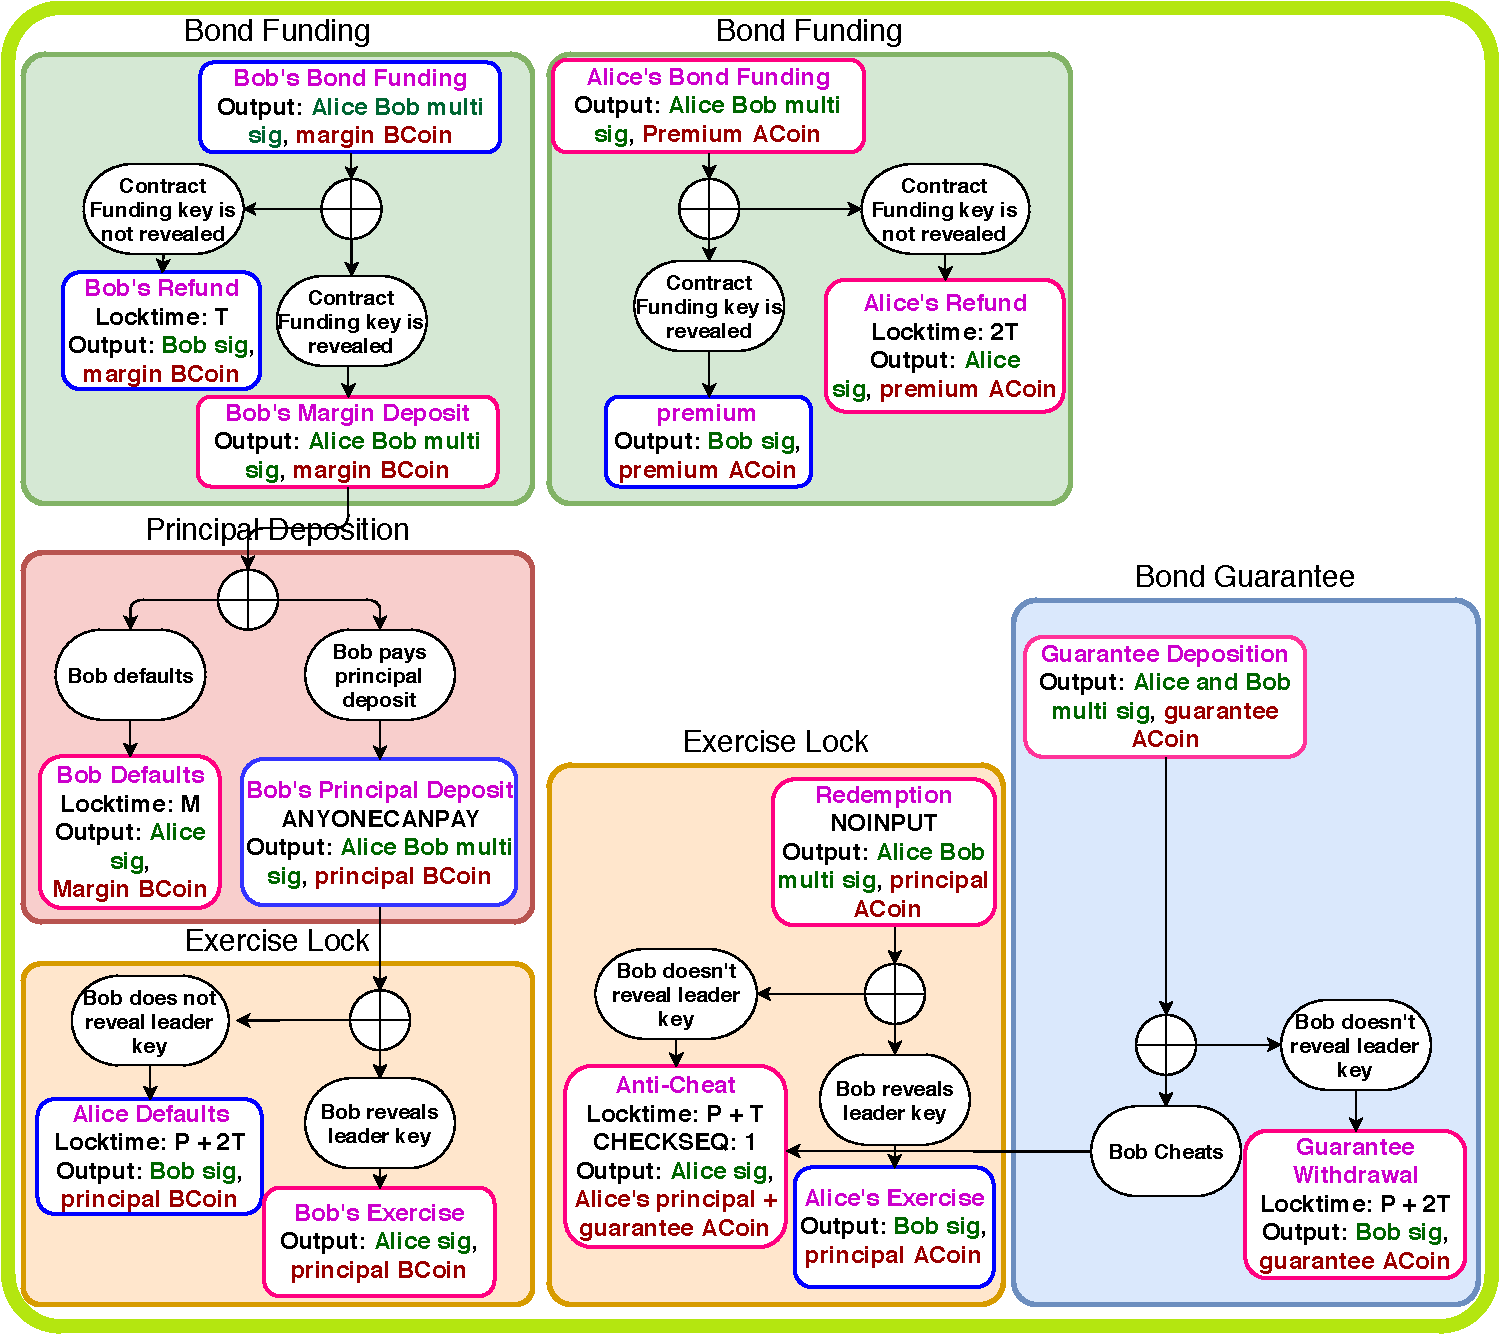
\includegraphics[width=\linewidth]{figures/bond-third.pdf}
  \caption{The ABCD across different chains. On each transaction, signatures, output amount and locktimes are specified. Bob's depositions are in BCoin and Alice's in ACoin. Pink-bordered transactions are broadcast by Alice and blue-bordered ones by Bob. For checkseq, block height is used. For locktimes, Unix timestamp is used. Upper transactions are broadcast earlier than the lower ones. If there is a line between two transaction, then the source transactions is considered to be an input of the destination transaction.}
  \Description{A cross-chain atomic bonded debt.}
  \label{fig:cross-chain-non-collat-bond}
\end{figure}

The difference between the intermediary ABD component and the ABCD primitive is addition of the guarantee withdrawal transaction \new{and its related funding transactios}. Whether Alice defaults or the bond is successfully \new{repurchased}, Bob has to broadcast the \new{\emph{guarantee withdrawal}} transaction. \new{Additionally, in the case of not revealing the \Aone} \new{key, Bob can take back his guarantee.} Other parts are the same in both procedures.
% The details of the ABCD is same as the intermediary ABD except for 